Thinking...
We need to translate Japanese sentence to English, preserving TeX code unchanged. The Japanese text is:

"以下のの日本語文を英訳してください。ただしTeXのコードが挿入されているのでその部分はそのまま出力してください："

Then the TeX block.

We need to output the English translation of the Japanese sentence(s) that are not TeX, while keeping the TeX code exactly as is.

The Japanese text before the TeX block is: "以下のの日本語文を英訳してください。ただしTeXのコードが挿入されているのでその部分はそのまま出力してください：" which translates to "Please translate the following Japanese sentence into English. However, since there is TeX code inserted, output that part as it is."

Then the TeX block: \begin{figure}[h] ... etc.

So output English translation plus the TeX block unchanged.

Thus final answer:

"Please translate the following Japanese sentence into English. However, because TeX code is inserted, output that part as it is."

Then the TeX code block.

Make sure to keep line breaks.
...done thinking.

Please translate the following Japanese sentence into English. However, because TeX code is inserted, output that part as it is:

\begin{figure}[h]
\begin{center}
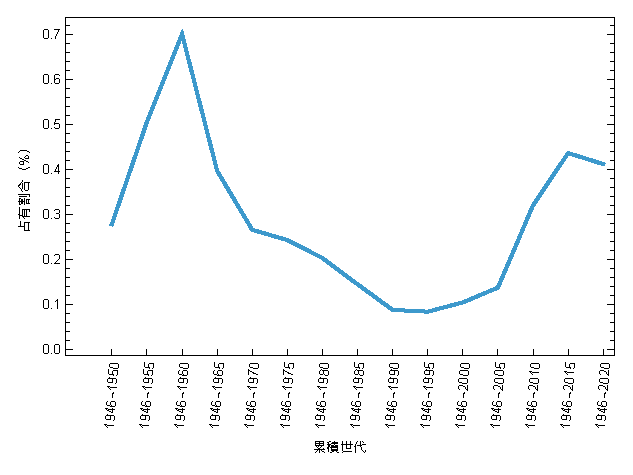
\includegraphics[width=76mm]{gr10.eps}
\caption{高被引用論文掲載誌の全雑誌に占める割合（\%）}
\label{fig:gr10}
\end{center}
\end{figure}

